
\begin{figure*}
  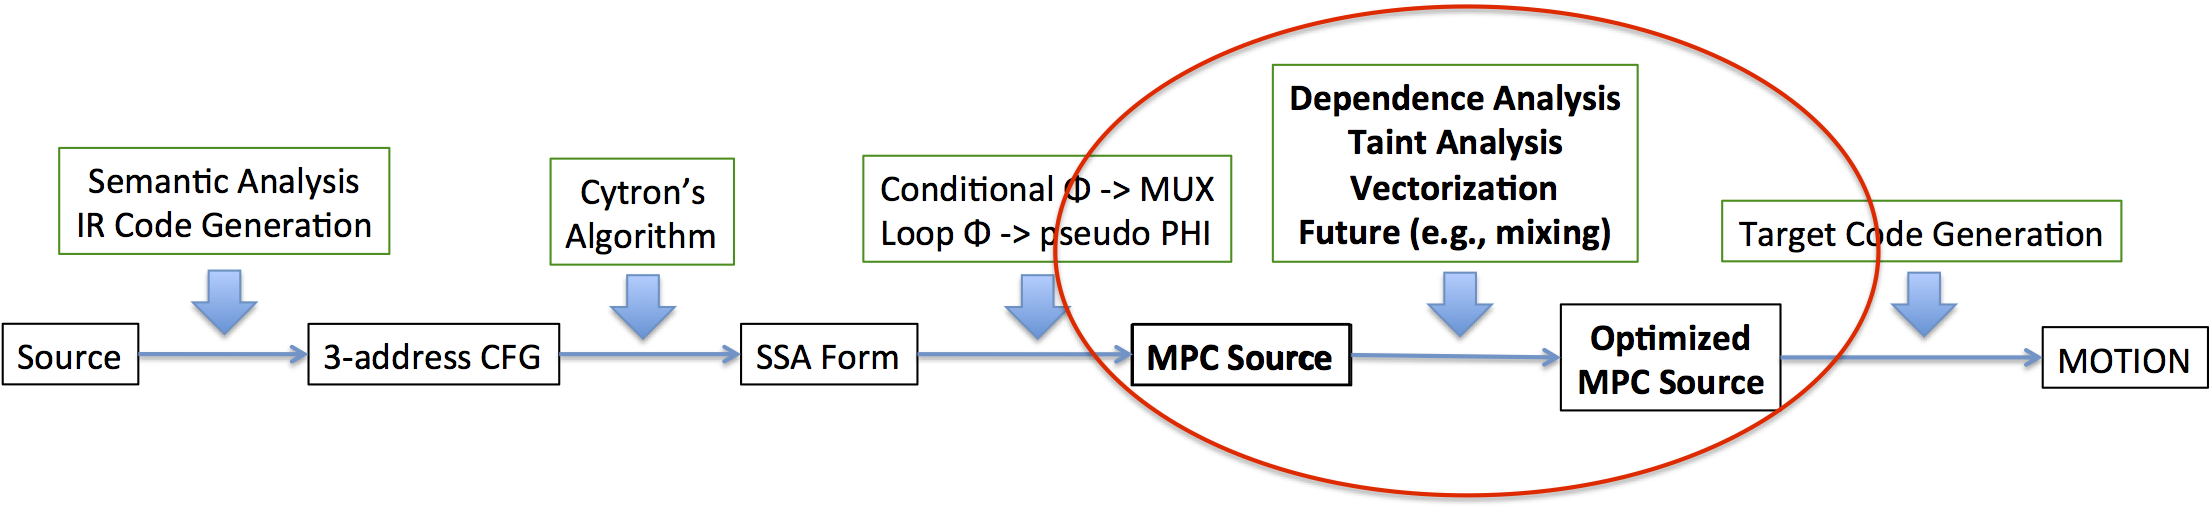
\includegraphics[width=1.0\linewidth]{figs_paper_SIMD/compiler_framework.png}
  \caption{Compiler Framework. \ana{Change figure since we are not doing div-and-conquer.}}
  \label{fig:compiler_framework}
\end{figure*}

\section{\bf Compiler Framework}
\label{sec:compiler}

\ana{Convention: use \texttt{shared, plain}, {\sf code}, $i$ and $I$ for counters outside of code.}

%We assume arbitrarily nested loops in the MPC-source IR and read-only arrays. We assume that loops range from 0 to some constant N. Arrays are linearized (row-major order as in MOTION) and accesses are via functions of the induction variables of the enclosing loops.

\figref{fig:compiler_framework} presents an overview of our compiler. This section describes the front-end phases of the compiler
and Section~\secref{sec:vectorization} describes our vectorization algorithm. \ana{We'll need a section on MOTION code gen too.}
%\ana{Need to state this more precisely.}

\subsection{Syntax and Semantic Restrictions}
\label{sec:syntax}

Source syntax is essentially standard IMP syntax as shown below:
%\begin{figure}[t]
{\small
\[
\begin{array}{l@{~~~~~}l}
  \begin{array}{l@{~}l@{~~~}l}
 e & ::= e \; \mathit{op} \; e \mid e \mid \x \mid  \texttt{const} \mid \texttt{A[$e$]} & \mathit{expression} \\
 % s &::= t \;\f & \mathit{field} \\
 %\md &::= t\;{\m}(t \;{\this}, \; t\;\x) \; \{\; \ol{t\;\y}\;\s;\;\return\;\y \; \}
 %                 & \mathit{method} \\
  s & ::= s;s \mid  & \mathit{sequence} \\
  & \x = e \mid \texttt{A[$e$]} = e \mid & \mathit{assignment \; stmt} \\
  & \texttt{for $i$ in range($I$)}: s \mid & \mathit{for \; stmt} \\
  & \texttt{if $e$: $s$ else: $s$} & \mathit{if \; stmt} \\
%   t &::= q \; {\sf C} & \mathit{qualified \; type}\\
%   q &::= \high \mid \poly \mid \low & \mathit{FlowCFL \; qualifier}\\
%    t' &::= q' \; \C & \mathit{field \; qualified \; type}\\
%   q' &::= \tainted \mid \poly & \mathit{field \; qualifier}\\

  \end{array}
\end{array}
\]
}
%\end{figure}

The syntax allows for array accesses, arbitrarily nested loops, and if-then-else control flow.
Expressions are typed $q \; \tau$, where qualifier $q$ and base type $\tau$ are:

{\small
\[
\begin{array}{l@{~~~~~}l}
  \begin{array}{l@{~}l@{~~~}l}
 \tau & ::= \texttt{int}  \mid \texttt{bool} \mid \texttt{list[int]} \mid  \texttt{list[bool]} & \mathit{base \; types} \\
  q & ::= \texttt{shared} \mid \texttt{plain} & \mathit{qualifiers} \\
  \end{array}
\end{array}
\]
}

The type system is mostly standard, and in our experience, a sweet spot between readability and expressivity.
The \texttt{shared} qualifier denotes shared values, i.e., ones shared among the parties and computed upon
under secure computation protocols; the \texttt{plain} qualifier denotes plaintext values. Shared lists denote
shared elements, but plaintext length. Subtyping is again as expected: $q_1 \; \tau <: q_2 \; \tau$
iff $q_1 <: q_2$ where $\texttt{plain} <: \texttt{shared}$. Thus, we can convert a plaintext value into a shared one,
but not vice versa.

Our compiler imposes certain semantic restrictions that it enforces throughout the various
phases of compilation. We note that in some cases, the restrictions
can be easily lifted and we plan to do so in future iterations of the work.

\begin{enumerate}
\item Loops are of the form $0 <= i < I$ and bounds are fixed at compile time.
It is a standard restriction in MPC that the bounds must be known at circuit-generation time.
\item Arrays are one-dimensional. N-dimensional arrays are linearized and accessed
in row-major order and at this point the programmer is responsible for linearization
and access. (This restriction can be easily lifted.)
\item Array subscrpts are plaintext values as specified by the rule:
\begin{semantics}
    \ntyperule{Array Access}{
%  \Gamma(\y) =  q_\y   \quad\quad \sigma(\f) = q_\f  \quad\quad \Gamma(\x) = q_\x \\
  \Gamma \vdash e : \texttt{plain int} \quad \Gamma \vdash \texttt{A} : q \; \texttt{list}[\tau] \quad \tau \in \{ \texttt{int}, \texttt{bool} \}
}{
  \Gamma \vdash \texttt{A[$e$]} : q \; \tau
}
\end{semantics}
The subscript $e$ is a function of the indices of the enclosing loops.
For read access, the compiler allows an arbitrary such function.
However, it restricts write access to \emph{canonical writes}, i.e., {\sf A[i,j,k] = ...}
where $i$, $j$ and $k$ loop over the three dimensions of {\sf A}.
Write access such as for example {\sf A[i,j+2] = ...} is not allowed.
%\item \ana{Add rules for logical ops}
%\item \ana{Add rules for arithmetic ops}
\item The final restriction involves MUX as expressed by the rule:
\begin{semantics}
    \ntyperule{MUX}{
%  \Gamma(\y) =  q_\y   \quad\quad \sigma(\f) = q_\f  \quad\quad \Gamma(\x) = q_\x \\
  \Gamma \vdash e_1 : q_1 \; \texttt{bool} \quad \Gamma \vdash e_2 : q_2 \; \tau \quad \Gamma \vdash e_2 : q_2 \; \tau \quad \tau \in \{ \texttt{int}, \texttt{bool} \}
}{
  \Gamma \vdash \texttt{MUX($e_1$,$e_2$,$e_3$)} : q_1 \vee q_2 \vee q_3 \; \tau
}
\end{semantics}
\end{enumerate}
Importantly, the arguments of MUX are restricted to base types, as passing array arguments
is not valid MOTION MPC. \ana{Check this.} This causes a slight inconvenience as we could not write
\begin{pythonn}
if e: A[i] = val
\end{pythonn}
Instead we had to write
\begin{pythonn}
if not(e): val = A[i]
A[i] = val
\end{pythonn}

We note that while the programmer writes
annotations at the level of IMP Source (recall \ana{ref to overview section}), the
annotations propagate through the transformations and are checked at the
level of MPC Source.

%\ana{Disadvantage of MUX}

For the rest of this section we write $i,j,k$ to denote the loop nest: $i$ is the outermost loop, $j$, is immediately nested in $i$, and so on until $k$
and we use $I,J,K$ to denote the corresponding upper bounds. We write $A[i,j,k]$ to denote canonical access
to an array element. In the program, canonical access is achieved via the standard row-major order formula: $(J*K)*i + K*j + k$.
To simplify the presentation we describe our algorithms in terms of three-element tuples $i,j,k$, however, discussion easily generalizes to
arbitrarily large loop nests.



\subsection{From IMP Source to SSA}

Our compiler translates from Source to SSA as follows:

\begin{enumerate}
  \item
        \textbf{Parsing}:
        Use Python's \texttt{ast} module to parse the input source code to a Python AST.
  \item
        \textbf{Syntax checking}:
        Ensure that the AST matches the restricted subset defined in Section~\secref{sec:syntax}.
        This step outputs an instance of the \texttt{restricted\_ast.Function} class, which represents our restricted subset of the Python AST.
  \item
        \textbf{3-address CFG conversion}:
        %\benjamin{TODO: Is this a good amount of detail?} \ana{This is good amount of detail for the Tech report. In the actual paper we'll shorten a lot and add pointers to the Tech report.}

        Convert the restricted-syntax AST to a three-address control-flow graph.
        To do this, first,
        add an empty basic block to the CFG and mark it as current.
        Next, for each statement in the restricted AST's function body,
        process the statement.
        Statements can either be for-loops, if-statements, or assignments (as in~\secref{sec:syntax}).
        Rules for processing each kind of statement are given below:
        \begin{enumerate}
          \item
                \textbf{For-loops}:
                Create new basic blocks for
                the loop condition
                (the \emph{condition-block}),
                the loop body
                (the \emph{body-block}),
                and the code after the loop
                (the \emph{after-block}).
                Insert a jump from the end of the current block to the condition-block.
                Then, mark the condition-block as the current block.
                Insert a for-instruction at the end of the current block with the loop counter variable and bounds from the AST.
                Next, add an edge from the current block to the after-block labeled ``FALSE'' and
                an edge from the current block to the
                body-block labeled ``TRUE''.
                Then, set the body-block to be the current block
                and process all statements in the AST's loop body.
                Finally, insert a jump to the condition-block and set the after-block as current.
          \item
                \textbf{If-statements}:
                Create new basic blocks for
                the ``then'' statements of the if-statement
                (the \emph{then-block}),
                the ``else'' statements of the if-statement
                (the \emph{else-block}),
                and the code after the if-statement
                (the \emph{after-block}).
                At the end of the current block,
                insert a conditional jump to the then-block or else-block
                depending on the if-statement condition in the AST.
                Next,
                mark the then-block as current,
                process all then-statements,
                and add a jump to the after-block.
                Similarly,
                mark the else-block as current,
                process all else-statements,
                and add a jump to the after-block.
                Finally, set the after-block to be the current block,
                and give it a \emph{merge condition} property equal to the condition of the if-statement.
          \item
                \textbf{Assignments}:
                In the restricted-syntax AST,
                the left-hand side of assignments
                can be a variable or an array subscript.
                If it is an array subscript, e.g., {\sf A[i] = x},
                change the statement to {\sf A = Update(A, i, x)}.
                If the statement is not already three-address code,
                for each sub-expression in the right-hand side of the assignment,
                insert an assignment to a temporary variable.
        \end{enumerate}
  \item
        \textbf{SSA conversion}:
        Convert the 3-address CFG to SSA with Cytron's algorithm.
\end{enumerate}

\subsection{From SSA to MPC Source} %: MUX Nodes and Pseudo $\phi$-nodes}

Once the compiler converts the code to SSA,
it transforms $\phi$-nodes that correspond to if-statements into MUX nodes.
From the 3-address CFG conversion step,
$\phi$-nodes corresponding to if-statements will be in a basic block
with the merge condition property.
For example, if $X_3 = \phi(X_1,X_2)$ is in a block with merge condition $C$,
the compiler transforms it into $X_3 = \mathit{MUX}(C, X_1, X_2)$.
Next, the compiler runs the dead code elimination algorithm from Cytron's SSA paper.

Next, the control-flow graph is \emph{linearized} into MPC Source,
which has loops but no if-then-else-statements.
This means that both branches of all if-statements are executed,
and the MUX nodes determine whether to use results from the then-block or from the else-block.
The compiler linearizes the control-flow graph with a variation of breadth-first search.
Blocks with the ``merge condition'' property are only considered
the second time they are visited,
since that will be after both branches of the if-statement are visited.
(The Python AST naturally gives rise to a translation where each conditional has exactly two targets,
and each ``merge condition'' block has exactly two incoming edges, a TRUE and a FALSE edge.
Thus, each $\phi$-node has exactly two multiplexer arguments, which dovetails into MUX.
This is in contrast with Cytron's algorithm which operates at the level of the CFG and allows for
$\phi$-nodes with multiple arguments.)
Each time the compiler visits a block,
it adds the block's statements to the MPC source.
If the block ends in a for-instruction,
the compiler recursively converts the body and code after the loop to MPC source
and adds the for-loop and code after the loop to the main MPC source.
If the block does not end in a for-instruction,
the compiler recursively converts all successor branches to MPC source and
appends these to the main MPC source.

Now, the remaining $\phi$-nodes in MPC source are the loop header nodes. We call these nodes \emph{pseudo} $\phi$-nodes
and we write \python{PHI} in MPC Source. A pseudo $\phi$-node $X_1 = $\python{PHI}$(X_0,X_2)$ in a loop header is evaluated
during circuit generation. If it is the 0-th iteration, then the $\phi$-node evaluates to $X_0$, otherwise, it evaluates to $X_2$.

%\ana{We need to double check that the following captures all cases of def-use edges.}

\subsection{Dependence Analysis}

The next steps construct the dependence graph and \ana{Add an intro here.}

\subsubsection{Def-use Edges}

The dependence graph has the following def-use edges:

\begin{itemize}
\item same-level edge $X\rightarrow Y$ where $X$ and $Y$ are in the same loop nest, say $i,j,k$. E.g., the def-use edge 9 to 10 in the Biometric MPC Source in Listing~\ref{tab:source_and_MPC_source_and_optimized_MPC_source} is a same-level edge. A same-level edge can be a back-edge in which case a $\phi$ node is the target of the edge.
E.g., 15 to 4 in Biometric is a same-level back-edge.
\item outer-to-inner $X\rightarrow Y$ where $X$ is in an outer loop nest, say $i$, and $Y$ is in an inner one, say $i,j,k$. E.g., 1 to 4 in Biometric forms is an outer-to-inner edge.
%A $\phi$-node can be a source or a target of an outer-to-inner forward edge.
\item inner-to-outer $X\rightarrow Y$ where $X$ is a $phi$-node in an inner loop nest, $i,j,k$, and $Y$ is in the enclosing loop nest $i,j$. E.g., the def-use from 8 to 12 gives rise to an inner-to-outer edge.
%E.g. $\texttt{sum}_0 = \phi(\texttt{sum}_1, 0)$ to $\texttt{c} = \mathit{CMP}(\texttt{sum}_0,\texttt{min}_0)$ is an inner-to-outer edge.
An inner-to-outer edge can be a back-edge as well, in which case both $X$ and $Y$ are phi-nodes with the source $X$ in a loop nested into $Y$'s loop (not necessarily immediately).

%Note that the source is \emph{always} a $\phi$-node of the $i,j,k$ loop and the target is in the immediately enclosing loop. The interpretation of this edge is that the use node $Y$ uses the definition made in the last iteration of the inner loop.
%\ben{The current representation of pseudo $\phi$-nodes shows them attached to the loop header (i.e. in the loop).  We may want to clarify that they are also evaluated at the loop's termination.}
%\item same-level back-edge $X\rightarrow Y$. $Y$ is a phi-node in the header of the loop and $X$ is a definition of the variable in the loop body. E.g., $\texttt{min}_1 = \mathit{MUX}(\texttt{c},\texttt{sum}_1,\texttt{min}_1)$ to $\texttt{min}_0 = \phi(\texttt{min}_1, 10000)$ in Biometric is a same-level back-edge.
%\item inner-to-outer back-edge $X\rightarrow Y$: $X$ and $Y$ are both $\phi$-nodes for some variable. The source $X$ is in a loop nested into $Y$'s loop (not necessarily immediately).

\item mixed forward edge $X\rightarrow Y$. $X$ is in some loop $i,j,k$ and $Y$ is in a loop nested into $i,j,k'$. We transform mixed forward edges as follows. Let $\x$ be the variable defined at $X$. We add a variable and assignment $\x' = \x$ immediately after the $i,j,k$ loop. Then we replace the use of $\x$ at $Y$ with $\x'$. This transforms a mixed forward edge into an "inner-to-outer" forward edge followed by an outer-to-inner forward edge. Thus, Basic Vectorization handles one of "same-level", "inner-to-outer", or "outer-to-inner" def-use edges.
 \end{itemize}

\subsubsection{Closures}

We define $\mathit{closure}(n)$ where $n$ is a phi-node. Intuitively, it computes the set of nodes (i.e., statements) that form a dependence cycle with $n$. The closure of $n$ is defined as follows:
\begin{itemize}
\item $n$ is in $\mathit{closure}(n)$
\item $X$ is in $\mathit{closure}(n)$ if there is a same-level path from $n$ to $X$, and $X \rightarrow n$ is a same-level back-edge.
\item $Y$ is in $\mathit{closure}(n)$ if there is a same-level path from $n$ to $Y$ and there is a same-level path from $Y$ to some $X$ in $\mathit{closure}(n)$.
\end{itemize}

\subsection{Taint Analysis}

We require that all inputs are marked as either shared or plaintext, however, we do not require any other qualifier annotations in the program. Then we infer if intermediate variables and expressions are shared through taint analysis with "taintedness" referring to the shared attribute.  Specifically, the compiler follows the following rules, which are standard in positive-negative qualifier systems (here \texttt{shared} is the positive qualifier and \texttt{plain} is the negative one):
\begin{enumerate}
\item Loop counters and array upper bounds are always \texttt{plain}.
\item If any variable on the right-hand side of an assignment is shared, then the assigned variable is \texttt{shared}.
%\item If all variables on the right-hand side of an assignment are plaintext, then the assigned variable is plaintext \ana{Will be covered by the last rule.}
\item Any variables that cannot be determined as shared via the above rules are \texttt{plain}.
\end{enumerate}

%The first two rules are standard for taint analysis, and the third rule follows from the MPC problem statement. \ben{Is the explanation for the third rule correct?}  \ana{Yes, that is exactly it!}
The final rule is needed in examples like the following. In the below snippet \texttt{sum!2} and \texttt{sum!3} form a dependency cycle and there is no \texttt{shared} value that flows to either one.
They are inferred as plaintext.
%cannot be marked as plaintext through simple taint analysis:
{\small
\begin{pythonn}
plaintext_array = [0, 1, 2, ...]
sum!1 = 0
for i in range(0, N):
    sum!2 = PHI(sum!1, sum!3)
    sum!3 = sum!2 + plaintext_array[i]
\end{pythonn}
}
%\ben{I think the above example is unnecessary and could be replaced by an explanation of how "untainted" variables are implicitly plaintext, but I couldn't think of a way to phrase that.}\ana{I left the example, we can leave it in the TR, remove from paper.}

When converting to MOTION code, any plaintext value used in the right-hand side of a shared assignment is converted to a shared value for that expression.
%\ben{Is this necessary to include?} \ana{Yes, that's important.}

Importantly, the taint analysis works on MPC Source, which lacks if-then-else control flow.
This significantly simplifies treatment as there is no need to handle conditionals and implicit flow.

\subsection{From (Optimized) MPC Source to MOTION}
\label{sec:MOTION}

MOTION supports FOR loops and SIMD operations, so translation from MPC source to MOTION C++ code is relatively straightforward.
% Variable naming
Our generated C++ uses the following variable-naming scheme: shared variables are named the same as in the MPC source with the \texttt{!} replaced with an underscore (e.g. \texttt{sum!2} would be translated to \texttt{sum\_2}).  Plaintext variables follow the same naming convention as shared variables but are prefixed with \texttt{\_MPC\_PLAINTEXT\_}.  The shared representation of constants are named \texttt{\_MPC\_CONSTANT\_} followed by the literal constant (e.g. the shared constant \texttt{0} would be named \texttt{\_MPC\_CONSTANT\_0}).

% Function preamble
The generated MOTION code begins with the declaration of all variables used in the function, including loop counters.  If a variable is a vectorized array, it is initialized to a correctly-sized array of empty MOTION shares.  Additionally, each plaintext variable and parameter has a shared counterpart declared.  Next, all constant values which are used as part of shared expressions are initialized as a shared input from party 0.  Finally, all plaintext parameters are converted used as shared inputs from party 0 to initialize their shared counterparts.

% Non-vectorized assignments and returns
Once the function preamble is complete, the MPC source is translated into C++ one statement at a time.  If there is no vectorization present in a statement, translation to C++ is straightforward: outside of Mux statements and array updates, non-vectorized assignments, expressions, and returns directly translated into their C++ equivalents.  Unvectorized Mux statements are converted to MOTION's Mux member function on the condition variable.  Array updates are translated into two C++ assignments: one to update the value in the original array and one to assign the new array.

\begin{table*}
\begin{tabular}{ccc}
\begin{minipage}{0.33\textwidth}
{\small
\begin{pythonn}
A[i] = val
\end{pythonn}
}
\end{minipage}

&

\begin{minipage}{0.33\textwidth}
{\small
\begin{pythonn}
A!2 = update(A!1, i, val)
\end{pythonn}
}
\end{minipage}

&

\begin{minipage}{0.33\textwidth}
{\small
\begin{cppp}
A_1[i] = val;
A_2 = A_1;
\end{cppp}
}
\end{minipage}

\\

IMP Source & MPC Source & MOTION Code
\end{tabular}
\caption{MOTION Translation: Array Updates}
\label{tab:motion_translation_array_updates}
\end{table*}

% Phi nodes and FOR loops
Phi nodes are broken into two components: the ``false'' branch which assigns the initial value of the phi node and the ``true'' branch which assigns the phi node's backedge.  The assignment of the false branch occurs right before the Phi node's enclosing loop.  Inside of the Phi node's enclosing loop, a C++ \texttt{if} statement is inserted to only assign the true branch of the phi node after the first iteration.  MPC FOR loops are converted to C++ FOR loops which iterate the loop counter over the specified range.  The loop counter is initialized before any phi nodes in the loop as they could rely on it; there is no other special handling of FOR loops.

\begin{table*}
\begin{tabular}{cc}
\begin{minipage}{0.5\textwidth}
{\small
\begin{pythonn}
for i in range(N):
   tmp = PHI(arr[i], val!0)
	 ...
\end{pythonn}
}
\end{minipage}

&

\begin{minipage}{0.5\textwidth}
{\small
\begin{cppp}
_MPC_PLAINTEXT_i = 0;
tmp = arr[_MPC_PLAINTEXT_i];
for (; _MPC_PLAINTEXT_i < _MPC_PLAINTEXT_N; _MPC_PLAINTEXT_i++) {
   if (_MPC_PLAINTEXT_i != 0) {
      tmp = val_0;
	 }
	 ...
}
\end{cppp}
}
\end{minipage}

\\

MPC Source & MOTION Code
\end{tabular}
\caption{MOTION Translation: FOR loop with Phi nodes}
\label{tab:motion_translation_for_loop}
\end{table*}

% SIMD representation
Vectorization is handled with utility functions to manage accessing and updating slices of arrays.  All SIMD values are stored in non-vectorized form as 1-dimensional \texttt{std::vector}s in row-major order.  Whenever a SIMD value is used in an expression, the utility function \texttt{vectorized\_access()} takes the unvectorized representation of a SIMD value, along with the size of each dimension and the requested slice's indices, and converts that slice to a MOTION SIMD value.  Because MOTION supports SIMD operations using the same C++ operators as non-SIMD operations, we do not need to perform any other transformations to the expression.  Therefore the translation of an expression containing SIMD values is identical to that of expressions without SIMD values once vectorized accesses are inserted.

Similarly, the \texttt{vectorized\_assign()} function assigns a (potentially SIMD) value to a slice of a vectorized array.  This operation cannot be done with a simple subscript as SIMD assignments will update a range of values in the non-vectorized representation.
\ben{Is the next sentence needed?  They can always check the implementation of vectorized\_assign() if they want to see specifics.}
The function takes the array being assigned to as a reference to update it in place so that any existing values are not lost.  SIMD values are never directly assigned to non-SIMD values.

\begin{table*}
\begin{tabular}{cc}
\begin{minipage}{0.5\textwidth}
{\small
\begin{pythonn}
sum!4[I] = ADD_SIMD(sum!3[I], p[I, j])
\end{pythonn}
}
\end{minipage}

&

\begin{minipage}{0.5\textwidth}
{\small
% Ben: This line is too long but I don't know how to break it well
\begin{cppp}
vectorized_assign(sum_4, {_MPC_PLAINTEXT_N}, {true}, {}, vectorized_access(sum_3, {_MPC_PLAINTEXT_N}, {true}, {}) + vectorized_access(p, {_MPC_PLAINTEXT_N, _MPC_PLAINTEXT_D}, {true, false}, {_MPC_PLAINTEXT_j}));
\end{cppp}
}
\end{minipage}

\\

MPC Source & MOTION Code
\end{tabular}
\caption{MOTION Translation: Assignment to SIMD value}
\label{tab:motion_translation_simd_assignment}
\end{table*}

% vectorized_update()
\ben{Technically this is semantically the same as non-vectorized update but we use a utility function to combine the steps into a single C++ statement - should it still be included?}
Updating SIMD arrays is also implemented differently from updating non-vectorized arrays.  Instead of separating the array update from the assignment of the new array, these steps are combined with the \texttt{vectorized\_update()} utility function.  This function operates identically to \texttt{vectorized\_assign()}, however it additionally returns the array after the assignment occurs.  This value is then used for the assignment to the new variable.

% raise_dim() implementation
\ben{The compiler and C++ internally uses ``lift'' as the terminology for raise\_dim(), but the paper does not :(...}
Raising the dimensions of an expression uses the \texttt{lift()} utility function which takes a lambda for the raised expression and the dimensions of the output.  The lambda accepts an array of integers representing the index along each of the dimensions being raised, and the translation of the expression which is being raised replaces each of the dimension index variables with the relevant subscript of this array.  There is also a special case of the \texttt{lift()} function which occurs when we are raising an array.  This case only occurs when the dimensionality of the array is equal to the first dimensions of the array (any dimension which is being lifted to which is not in the array is after every dimension in the array) \ben{I don't know how to phrase the previous sentence more concisely}.  In this case, the array is simply extended along the new dimensions (if the array is already correctly sized it is returned as is).

% Ben (note as comment since tables aren't fixed placement): I only include the translation of the expression itself (instead of an assignment) since the assignment includes the extra junk from a vectorized_assign.  Also none of the raise_dims in biometric use the dimension index which I think is the most interesting/important part of the lift expression translation so I made up a toy example.
\begin{table*}
\begin{tabular}{cc}
\begin{minipage}{0.5\textwidth}
{\small
\begin{pythonn}
raise_dim(i + j, (i:N, j:M))
\end{pythonn}
}
\end{minipage}

&

\begin{minipage}{0.5\textwidth}
{\small
\begin{cppp}
lift(std::function([&](const std::vector<std::uint32_t> &idxs){return idxs[0] + idxs[1];}), {_MPC_PLAINTEXT_N, _MPX_PLAINTEXT_M})
\end{cppp}
}
\end{minipage}

\\

MPC Source & MOTION Code
\end{tabular}
\caption{MOTION Translation: Raising dimensions}
\label{tab:motion_translation_raise_dim}
\end{table*}

% drop_dim() implementation
Dropping dimensions use the \texttt{drop\_dim()} and \texttt{drop\_dim\_monoreturn()} utility functions.  They function identically but the latter returns a scalar for the case when the final dimension of an array is dropped.  These functions take the non-vectorized representation of an array, along with the dimensions of that array, and return the array with the final dimension dropped.
\ben{drop\_dim() taking the true branch of phi node values doesn't need to be covered here, right?}

% Shared/plaintext conversions
\ben{Ishaq or Vassilis: please check over this paragraph... I don't want to make some mistake about MOTION's capabilities.}
Currently, our compiler only supports the \texttt{Bmr} and \texttt{BooleanGMW} protocols as MOTION does not implement all operations for other protocols \ben{Should that go here?}.  MOTION does not support publicly-known constants for these protocols, so all conversions from plaintext values to shares are performed by providing the plaintext value as a shared input from party 0.  Due to this limitation, our translation to MOTION code attempts to minimize the number of conversions into a plaintext value.  This is accomplished by creating a shared copy of each plaintext variable and updating that copy in lock-step with the plaintext variable.  Since variables are often initialized to a common constant value (e.g. 0), this approach decreases the number of input gates by only creating a shared input for each constant.  Loop counters must still be converted to a shared value on each iteration that they are used, however we only output this conversion when necessary to prevent loops where the counter is not used in a shared expression from increasing the number of input gates.

% Tons of copies != runtime costs
Due to the SSA translation phase as well as the various conversions to and from SIMD values which our utility functions perform, our generated MOTION code often includes many copies of arrays and scalar values.  These copies do not incur a runtime cost as the arrays simply hold pointers to the underlying shares, so no new shares or gates are created as a result of this copying. \ben{Is there anything else to say here?  Should this be placed somewhere else?}